%%%%%%%%%%%%%%%%%%%%%%%%%%%%%%%%%%%%%%%%%%%%%%%%%%%%%%%%%%%
% EPFL report package, main thesis file
% Goal: provide formatting for theses and project reports
% Author: Mathias Payer <mathias.payer@epfl.ch>
%
% This work may be distributed and/or modified under the
% conditions of the LaTeX Project Public License, either version 1.3
% of this license or (at your option) any later version.
% The latest version of this license is in
%   http://www.latex-project.org/lppl.txt
%
%%%%%%%%%%%%%%%%%%%%%%%%%%%%%%%%%%%%%%%%%%%%%%%%%%%%%%%%%%%
\documentclass[a4paper,11pt,oneside]{report}
% Options: MScThesis, BScThesis, MScProject, BScProject
\usepackage[BScProject,lablogo]{EPFLreport}
\usepackage{xspace}
\usepackage{listings}
\usepackage{caption}
\usepackage{subcaption}

\renewcommand{\lstlistingname}{Configuration}
\lstset{
  basicstyle=\footnotesize\ttfamily,
  columns=flexible,
  literate={-}{-}1,
  breaklines=true,
}
\lstset{captionpos=b}
\AtBeginDocument{\def\chapterautorefname{Chapter}}
\AtBeginDocument{\def\sectionautorefname{Section}}%
\AtBeginDocument{\def\subsectionautorefname{Subsection}}%
%

\title{Smallworld: Gossiping with Raspberry Pis Locally}
\author{Romain Küenzi (continued by Guilhem Niot)}
\supervisor{Dr. Erick Lavoie}
\adviser{Professor Anne-Marie Kermarrec}

\newcommand{\sysname}{FooSystem\xspace}

\begin{document}
\maketitle

\maketoc

%%%%%%%%%%%%%%%%%%%%%%
\chapter{Introduction}
%%%%%%%%%%%%%%%%%%%%%%

In high-income countries, the ubiquity of Internet access encourages users to rely on online centralized services when direct connectivity between devices would be sufficient: when exchanging files or collaborating on shared documents for example. This increases the energy usage of the network and cloud infrastructure; it also introduces privacy compromises, as many of the online services monetize user behavior and interests to cover their operating costs.

In low-income countries, Internet connectivity may be unaffordable to many so direct connectivity may become the only affordable option. And in situations of humanitarian crises, the required telecommunication networks may simply no longer be available so direct connectivity may become the only possible option.

While mobile devices used in all the previous situations most often have the required physical communication capabilities for direct connectivity, through protocols such as Wi-Fi \cite{wifi2016} and Bluetooth \cite{bluetooth}, different mobile vendors implement different higher-level protocols that are not interoperable. As an example, Apple devices use their own proprietary protocol, AWDL \cite{appleAWDL}, whereas Android devices use the Wi-Fi Direct standard \cite{wifiDirect}.

% Feels incomplete
The objective of this project is to tackle afore mentioned issues: simplify device-to-device communication in an affordable way. Connection should require minimal interaction from the users and, once it is established, allow automatic sharing of data between them using peer-to-peer protocols and applications.

% Okayish
With that goal in mind, we will first have to make a few technology choices to make our solution as available as possible and ideally compatible with all existing devices. To achieve this compatibility, the first choice is an hardware platform: the Raspberry Pi. Then we need to choose standards communications protocols. At the physical layer we will rely on Wi-Fi, which enables the usage of the the Internet protocol suite in higher layers. We will then demonstrate in which scenario the resulting device can be used. The actual solution will be described in two steps, first listing all the required software tools, then explaining the implementation of a simple script that enables to create the communication networks. Finally we will demonstrate the effective usage of the device with an existing peer-to-peer application called Secure-Scuttlebutt \cite{tarr2019secure}.


%%%%%%%%%%%%%%%%%%%%
\chapter{Technology Choices}
 \label{chap:technology}
%%%%%%%%%%%%%%%%%%%%

This first chapter describes and justify the technology choices that were made, showing their advantages and explaining why other solutions were dismissed.

\section{Hardware Platform}

\emph{Raspberry Pis} are single-board computers developed by the \emph{Raspberry Pi Foundation} whom have an objective to make digital technologies accessible and affordable. Multiple models are available, with the most standard coming at a price of 35\$. The particular model used in this project is the \emph{Raspberry Pi Zero W}. It is a smaller and cheaper (10\$) board and therefore has a bit less computing power, but it still includes Wi-Fi and Bluetooth capabilities. With this the affordability requirement is met\footnote{All the Raspberry Pi products and their reference prices can be found on the Raspberry Pi website at \url{https://www.raspberrypi.org/}}.

Choosing the RPi also came with other various advantages in the research and implementation of a solution. First, finding ressources is fairly simple as the RPi has a big community of users and a complete online documentation. The board used in this project has everything we need for multiple connectivity options, namely micro-USB, Wi-Fi and Bluetooth modules. Other boards also have USB and Ethernet ports. As mentioned earlier, the RPi is a single-board computer and it usually runs on the \emph{Raspberry Pi OS}, an operating system based on Debian. That gives access to the standard tools you have on any computer running a Linux distribution.

Lastly, having a dedicated device for direct connectivity might sound unnecessary when the devices you own already have the capabilities to communicate together, but as already pointed out in the introduction, devices tend to implement different incompatible protocols. As shown in \autoref{fig:compatGraph}, if you want to allow connectivity between any devices, you have to solve a complex many-to-many compatibility graph, whereas if you use a dedicated device you only have to solve one-to-many.

\begin{figure}
  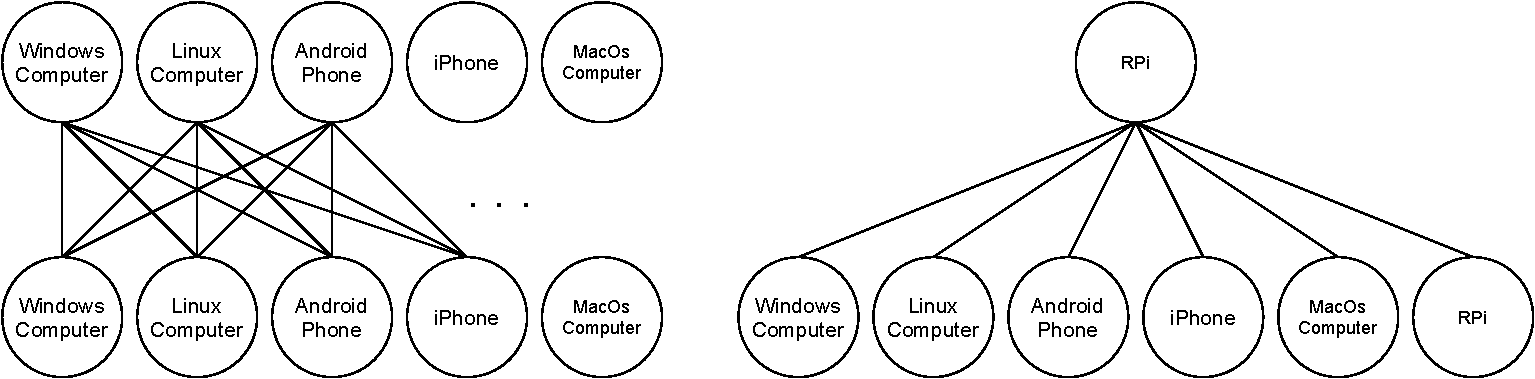
\includegraphics[width=\linewidth]{figures/compatibilityGraph.pdf}
  \caption{Many-to-Many vs. One-to-Many compatibility graph}
  \label{fig:compatGraph}
\end{figure}

\section{Communication Protocol: Wi-Fi and IP}

The next step is to choose which communication protocol to use. Always aiming for simplicity and maximum compatibility, the best solution is to use what already exists and is widely implemented: Wi-Fi and the \emph{Internet Protocol} (IP). These choices come with a lot of advantages.

For end users, Wi-Fi is a technology they are used to, so it should not be hard to understand how the device work. The wide usage of Wi-Fi and IP also made it easier to find ressources, tools and already compatible applications.

Wi-Fi network are used to create \emph{Local Area Networks} (LAN). IP is used for giving addresses on the Internet but it also does it in LAN. This address is used to communicate with other devices on the Internet, but it works the same in LAN, if the IP of another device is known, you can start sending it messages. On the Internet, the \emph{Network Address Translation} (NAT) performed by home
routers makes it complicated to locate a specific device. But on a LAN there exists multiple ways to do this, for example \emph{Avahi}\footnote{Avahi facilitates service discovery on LAN : \url{https://avahi.org/}} lets you announce to everyone that you are available on the network to deliver specific services (and therefore communicate). SSB, the protocol we will use in \autoref{chap:ssb} to verify the functioning of the device, also implements a way to discover all peers on a LAN by broadcasting UDP messages.

To facilitate Wi-Fi setup on our device, we used the \emph{Wi-Fi Protected Setup} (WPS) standard \cite{wifi2016}. It enables devices to create secure connections that require less configuration steps from the users. In our case, we use the push-button method, which sets up a Wi-Fi connection between the host and the client when a button is pressed on both devices.

\section{Discarded Option: Bluetooth}

The other option available for wireless communication is Bluetooth but the idea of using it was quickly dismissed. It is not appropriate for the following reasons:

\begin{itemize}
  \item It has a low transfer rate (< 2 Mbits). We want to be able to transmit any kind of data and it includes potentially large files. Wi-Fi as available on the RPi Zero W can transmit up to 54 Mbit/s and other devices with more recent Wi-Fi chips can go above this limit.
  \item Bluetooth is designed to implement application-specific protocols in higher layers which means that, among other things, it does not work easily with IP networking.
\end{itemize}

\section{Wi-Fi or Wi-Fi Direct}

Initially, one of the objectives was to implement a solution that used Wi-Fi Direct. The main advantage would have been a simpler user experience. Wi-Fi Direct removes the need to choose which device hosts the network, as the protocol determines it automatically. The resulting device would have had a single use case: connect to another device. In fact WPA Supplicant, the tool used to manage Wi-Fi networks (described in more detail in \autoref{chap:tools}), offers Wi-Fi Direct functionalitie. But even after some research we were not able to connect devices with it. In the end, loosing this option was not critical because, despite being broadly implemented by Android phones, it is not available on iOS devices. Linux PCs should be capable to use Wi-Fi Direct through WPA Supplicant but they do not always have a user interface to use it. In any case, Wi-Fi Direct could always be implemented later as an optional feature.

\section{Ethernet-over-USB}

The Raspberry Pi Zero W, along with \emph{Raspberry Pi 4}, also offers the possibility to implement Ethernet-over-USB\footnote{Other models of Raspberry Pis do not offer this feature}. Ethernet, like Wi-Fi, works well with the Internet Protocol. As it can be implemented with just a few configuration changes on the RPi, this option is also set up. However the compatibility is not as good as Wi-Fi. It was only verified to work with a Linux laptop. We also tested it with a Windows desktop and an Android phone and it did not work. Although it might work with some more configuration on these devices, it does not fill our criteria of simplicity. This functionality has not been tested with other devices.


%%%%%%%%%%%%%%%%
\chapter{User Experience}
\label{chap:user}
%%%%%%%%%%%%%%%%

This chapter presents a scenario that highlights all the uses of the device that we envisioned. The scenario assumes that each participant uses an application that replicates the data they want to share to all their friends, and also their own devices. We will explain in more detail
in Chapter 5 how this scenario can be implemented with the SSB protocol \cite{kermarrec2020gossiping}.
For now, we present the scenario from the perspective of end-users, without
reference to SSB-specific implementation details. On the figures, arrows indicate that two devices are connected to each other and the device it points to hosts the network. Doted arrows indicate when data flows from one device to another. For RPis, blue dots indicate that it is connected to a Wi-Fi network and green dots indicate that it is hosting its own Wi-Fi network.

Alice likes to take a lot of photos on her phone and share them with friends. At home she always connects all her devices to the Wi-Fi network. As \autoref{fig:aliceHome} shows, it is quite convenient because her photos get replicated to both her laptop and her RPi. With her laptop she can edit them, create albums, \ldots, and with her RPi she can easily share them with friends when they meet. This show the first usage of the device where it is simply connected to an existing network and synchronizes with other devices on the network.

When she goes out to meet friends she takes her RPi along to be able to share her photos. Today, she meets two friends, Bob and Charlie, and during the discussion, she talks about the last pictures she took. Bob and Charlie really want to see the photos so they all bring out their devices. Bob chooses to enable the Access Point on his device so he can connect his phone easily and take a look at Alice's photos right away. The other two connect their devices to Bob's network. As shown in \autoref{fig:meeting} every device receives the pictures including Bob's phone, so he can take a look at the pictures with Charlie. This illustrates two other uses of the device: they can connect to each other, and other devices can be connected to them in the same way these other devices connect to any Wi-Fi network. Once connected, all the devices are able to communicate.

During their meeting, Charlie and Alice also received some data from Bob. After the other two leave, Charlie still has some work to do so he takes out his laptop. A bit later, while taking a break, he recalls that Bob likes to write blog posts about his favorite turtle pet, so he brings out his RPi and USB cable and plug his device to his laptop. As shown in \autoref{fig:charlieBreak}, he receives all the data he got earlier from Alice and Bob on his laptop. As expected, Bob wrote a new blog post, so Charlie spends the rest of his break reading funny stories about Bob's turtles. This show the last connection option using a USB cable. The laptop connects to the RPi network in the same way it connects to a network using an Ethernet cable, and the two devices can communicate.

\begin{figure}
    \begin{subfigure}{0.5\textwidth}
        \centering
        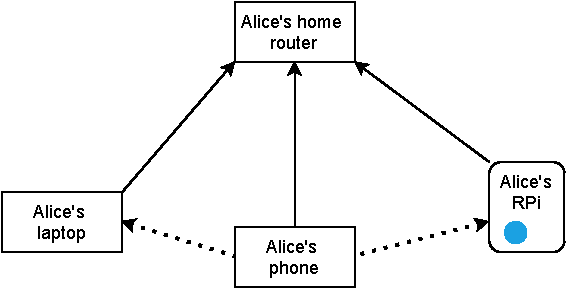
\includegraphics[height=4cm]{figures/scenarioAliceHome.pdf}
        \caption{Alice's home}
        \label{fig:aliceHome}
    \end{subfigure}%
    % ~
    \begin{subfigure}{0.5\textwidth}
      \centering
      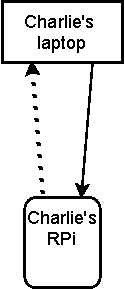
\includegraphics[height=4cm]{figures/scenarioCharlieBreak.pdf}
      \caption{Charlie's break}
      \label{fig:charlieBreak}
    \end{subfigure}
    \bigbreak
    \begin{subfigure}{\textwidth}
      \centering
      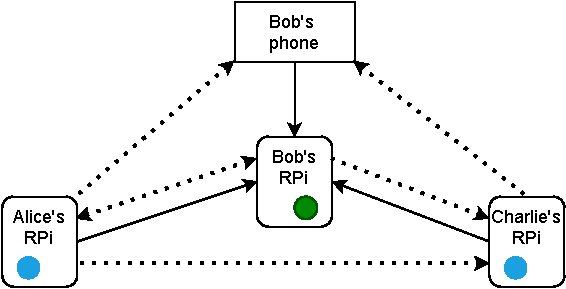
\includegraphics[height=4cm]{figures/scenarioMeeting.pdf}
      \caption{Friends meetup}
      \label{fig:meeting}
    \end{subfigure}
    \caption{}
\end{figure}


%%%%%%%%%%%%%%%%%%%%
\chapter{Design and Implementation of Connectivity}
%%%%%%%%%%%%%%%%%%%%

\section{Software Tools}
\label{chap:tools}

The first step toward the construction of a solution is to find the appropriate tools to manage the technologies mentioned in \autoref{chap:technology}. Here is a list of the tools used to manage connectivity on the Raspberry Pi:

\textbf{WPA Supplicant}\footnote{\url{https://w1.fi/wpa_supplicant/}} is a service (or "daemon" program) that runs in the background to manage wireless connections. It can be controlled through a C library (to develop your own frontend) but also comes with a text-based frontend (wpa\_cli) and a GUI (wpa\_gui). It is made to support most Wi-Fi related standards.

\textbf{Hostapd}\footnote{\url{https://w1.fi/hostapd/}} is a service to create and manage Wi-Fi access points and authentication. It also comes with a text-based frontend (hostapd\_cli).

\textbf{DHCP} is the protocol used to assign addresses on an IP network. To connect to existing IP networks, a DHCP client is necessary so the RPi comes with a default DHCP client called \emph{dhcpcd}\footnote{\url{https://roy.marples.name/projects/dhcpcd/}}. In some situations, we want the RPi to control a network, therefore it needs to assign itself and other devices on the network an IP address. \emph{Dnsmasq}\footnote{\url{https://thekelleys.org.uk/dnsmasq/doc.html}} provides multiple network infrastructure tools for small networks, including an easy to configure DHCP server that we use to assign IP addresses on the networks we create with the RPi.

\textbf{Systemd}\footnote{\url{https://systemd.io/}} is the service manager for Debian. It starts background scripts on boot and manage them during execution: we use it to run WPA Supplicant,
the Smallworld script we developed (\autoref{chap:impl}), and the hostapd service.

Two of these tools, hostapd and dnsmasq, are not preinstalled on the RPi. They have to be downloaded and installed with \emph{aptitude}, the Debian package manager, with the commands in \autoref{cmd:install}.

\begin{figure}
\begin{lstlisting}[label=cmd:install, caption=Hostapd and dnsmasq installation]
    apt-get update
    apt-get install hostapd dnsmasq
    # Unmask hostapd with systemd
    systemctl unmask hostapd
\end{lstlisting}
\end{figure}


\section{The Smallworld script}
\label{chap:impl}

Smallworld is a python script that establishes and monitors wireless connections between devices in close proximity. It runs as a background service that starts when the RPi boot. The script, along with example configuration files, is available at \url{https://github.com/rkuenzi-epfl/smallworld}.

\subsection{Design}

The current design comprises a Raspberry Pi Zero W with two push buttons, two 220 Ohm resistors and two LEDs connected to its GPIOs. \autoref{fig:electricalSchema} illustrates the electrical schema of the connected components. The buttons control the device and the LEDs give feedback on its current connection status. The AP button is connected to GPIO 13, and the LED giving feedback for the AP is connected to GPIO 19. The WPS button is connected to GPIO 6. The LED on GPIO 26 gives feedback on the connection status of the device in both host and client mode.
\begin{figure}
  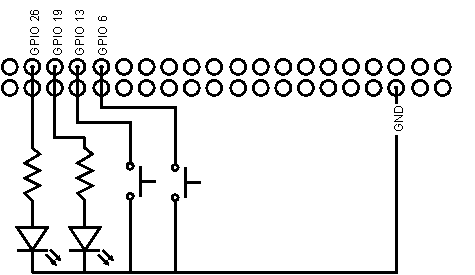
\includegraphics[width=\linewidth]{figures/electricalSchema.pdf}
  \caption{Electrical schema of the final device}
  \label{fig:electricalSchema}
\end{figure}


\autoref{fig:stateMachine} illustrates the complete behavior of the daemon. When the RPi starts, the \emph{Access Point} (AP) is disabled. The device eventually connects to known Wi-Fi networks listed in the \verb|wpa_noAP.conf| file if any is available. When the user presses the WPS push-button, the RPi tries to connect to an existing Wi-Fi network. The \emph{Connection State} LED blinks until it finds an available Wi-Fi to connect to then stays on if the connection is successful. If it does not find a Wi-Fi waiting for a WPS connection, it stops searching and times out after two minutes. When pressing on the AP button, the device starts its own Wi-Fi network (and turn on the AP LED). Any Wi-Fi device can connect to this AP the same way they connect to a home network as long as the passphrase is known. If the other device implements a WPS push-button, it can also be connected by starting a WPS search on both devices. When the AP is enabled the \emph{Connection State} LED stays on as long as there is at least one device connected to the network, and always blinks during WPS discovery.
\begin{figure}
  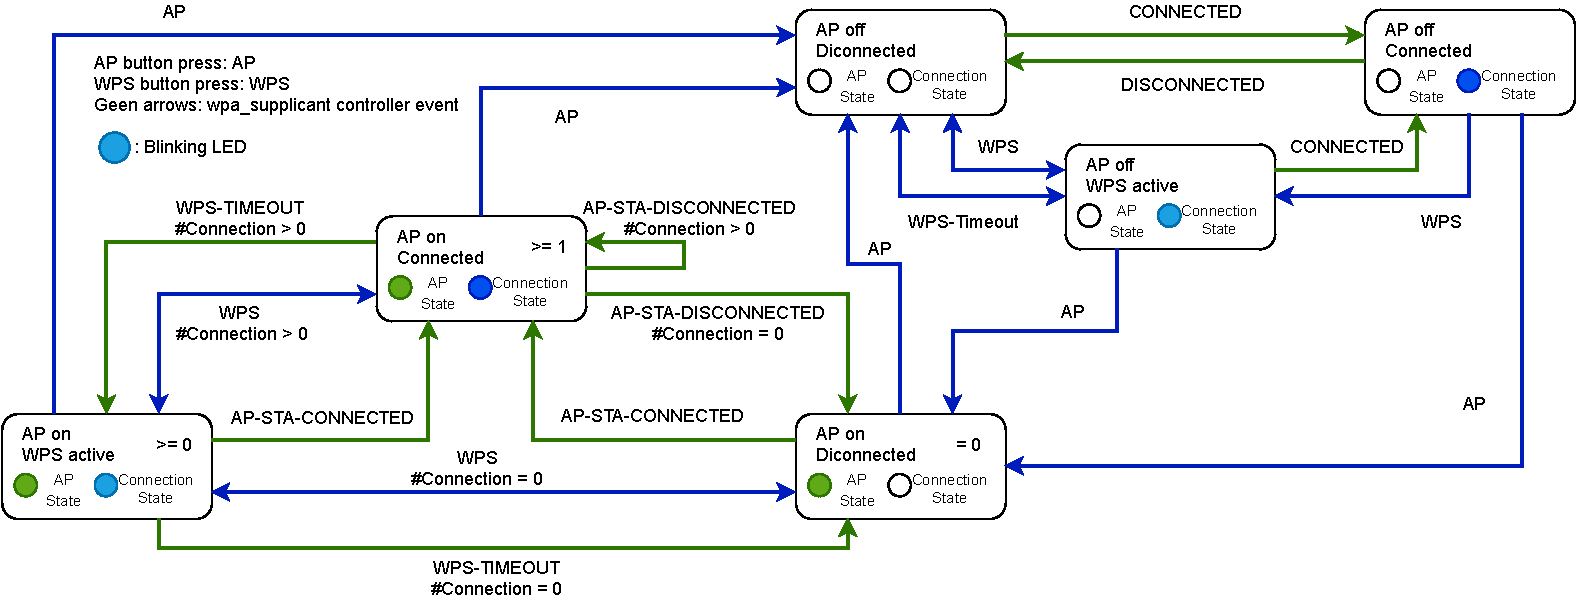
\includegraphics[width=\linewidth]{figures/stateMachine.pdf}
  \caption{Smallworld state machine}
  \label{fig:stateMachine}
\end{figure}

\subsection{Configuration}
\label{chap:conf}

An important part of the solution relies on specific usages and configurations of the tools mentioned in \autoref{chap:tools}. The script sometimes relies on "default behaviors" resulting from these specific configurations, which make them all the more important. Configurations presented here are meant as examples and most of them can be modified to the user preferences.

First we configure the DHCP client and server\footnote{Files for both dhcpd and dnsmasq are found under the /etc folder and follow the <software\_name>.conf convention for their configuration filenames}. Dnsmasq makes the server configuration quite easy. After its installation you add the following line \verb|dhcp-range=wlan0,192.168.4.2,192.168.4.20,255.255.255.0,24h| to the dnsmasq configuration file. In order, the arguments define the followings: interface to distribute the addresses on, first address to serve, last address to serve, address mask and leasing time. A DHCP request happens whenever the RPi creates or connects to a network, so the DHCP client needs to be configured for both of these situations. \autoref{conf:dhcpcd} shows the configuration for the DHCP client. The default configuration for \verb|interface wlan0| runs a standard DHCP request, but if it fails it fallbacks to \verb|profile ap_wlan0|. That happens when the RPi creates its own Wi-Fi network. The ap\_wlan0 profile has to use the first address on the subnet defined by dnsmasq. This configuration should be appended to the dhcpcd configuration file.

\begin{figure}
\begin{lstlisting}[label=conf:dhcpcd, caption=DHCP client configuration]
    profile ap_wlan0
    static ip_address=192.168.4.1/24
    static routers=192.168.4.1
    nohook wpa_supplicant

    interface wlan0
    fallback ap_wlan0
\end{lstlisting}
\end{figure}

Then we configure WPA Supplicant. The default WPA Supplicant configuration is in \verb|/etc/wpa_supplicant/wpa_supplicant.conf|, but we do not modify it directly. Instead the smallworld script uses two configuration files, \verb|wpa_AP.conf| and \verb|wpa_noAP.conf|, that overwrite the default WPA Supplicant configuration during execution. The base for both of them is shown in \autoref{conf:wpa_supplicant}. If we want the RPi to automatically connect to specific Wi-Fi networks we can add configurations for those in \verb|wpa_noAP.conf|. \autoref{conf:network_template} gives a template to configure a standard WPA2 network that should work for most home networks\footnote{We can append as much of these network configurations as we want to the file and WPA Supplicant will connect whenever one of them is available.}. However \verb|wpa_AP.conf| has to stay empty for the Access Point to start properly\footnote{We did not manage to run hostapd without running WPA Supplicant with this empty configuration file... but it might be possible.}.

\begin{figure}
\begin{lstlisting}[label=conf:wpa_supplicant, caption=Base WPA Supplicant configuration file, numbers=left]
    ctrl_interface=DIR=/var/run/wpa_supplicant GROUP=netdev
    update_config=0
    country=CH
\end{lstlisting}
\centering
\end{figure}

\begin{figure}
\begin{lstlisting}[label=conf:network_template, caption=Home network configuration template]
    network={
      ssid=<network_ssid>
      psk=<network_password>
    }
\end{lstlisting}
\end{figure}

The next step is to configure hostapd. \autoref{conf:hostapd_conf} gives a complete example to setup a Wi-Fi network using WPA2 security, which is equivalent to what is used for home networks. Otherwise, only lines 11 to 14 are specific to the implementation, because they enable WPS push-button. The only things to complete in the file are the \verb|<network_ssid>| and \verb|<network_password>|.

\begin{figure}
\begin{lstlisting}[label=conf:hostapd_conf, caption=Complete Access Point configuration, numbers=left]
    country_code=CH
    interface=wlan0
    ssid=<network_ssid>
    hw_mode=g
    channel=7
    macaddr_acl=0
    auth_algs=1
    ignore_broadcast_ssid=0
    wpa=2
    wpa_passphrase=<network_password>
    wpa_psk_file=/etc/hostapd/hostapd.psk
    wps_state=2
    ap_setup_locked=1
    config_methods=label display push_button keypad
    ctrl_interface=/var/run/hostapd
    ctrl_interface_group=netdev
    eap_server=1
    wps_pin_requests=/var/run/hostapd.pin-req
    wpa_key_mgmt=WPA-PSK
    wpa_pairwise=TKIP
    rsn_pairwise=CCMP
\end{lstlisting}
\end{figure}

Finally, we write \autoref{conf:service} in \verb|/lib/systemd/system/smallworld.service|. It runs the smallworld script on boot and restart if it stops for any reason. For this service to work we have to put a few files in the right place: \verb|wpa_AP.conf| and \verb|wpa_noAP.conf| should be moved to the \verb|/etc/smallworld/| folder and \emph{smallworld}, as well as another script called \emph{smallworldForwardEvent}, should be moved to \verb|/usr/sbin/|. Once everything is in place, running \verb|systemctl enable smallworld| will start the script at every boot.

\begin{figure}
\begin{lstlisting}[label=conf:service, caption=Service file for smallworld, numbers=left]
    [Unit]
    Description=Smallworld script
    After=multi-user.target

    [Service]
    Type=simple
    StandardOutput=journal
    RuntimeDirectory=smallworld
    WorkingDirectory=/run/smallworld
    ExecStart=/usr/sbin/smallworld
    Restart=always

    [Install]
    WantedBy=multi-user.target
\end{lstlisting}
\end{figure}

\subsection{Implementation}

First, the \emph{smallworld} script connects to the WPA Supplicant control interface to react when an event happens, such as connection/disconnection from a Wi-Fi network or any WPS event. The WPA Supplicant client offers a method to run a script, with the event informations as parameters, every time an event happens with the Wi-Fi controller (\autoref{cmd:cli}, line 8). This method is used to run the second script, \emph{smallworldForwardEvent}. This script sends a UDP message on the local machine with the informations received from WPA Supplicant. The smallworld script runs a UDP server to receive theses messages and react accordingly.

The smallworld script also reacts to user interactions and gives feedback on its state. It uses the \emph{GPIO Zero} package\footnote{Part of the default installation of the Raspberry Pi OS, documentation is available at \url{https://gpiozero.readthedocs.io/en/stable/}} to handle the RPi GPIO pins and consequently, buttons and LEDs.

When the user enables the AP by pressing the appropriate button the following sequence happens:
\begin{enumerate}
  \item WPA Supplicant configuration file is overwritten with \verb|wpa_AP.conf|.
  \item The script forces WPA Supplicant to reread its configuration file (\autoref{cmd:cli}, line 10).
  \item Hostapd service is turned on with the command written in \autoref{cmd:systemd}.
  \item Hostapd starts forwarding its control interface events (\autoref{cmd:cli}, line 17).
  \item It turns the AP LED on.
\end{enumerate}

When enabling the AP, reconfiguring WPA Supplicant has various useful side effects that depend on the configurations described in \autoref{chap:conf}. It disconnects the Wi-Fi, which is necessary to allow hostapd to create its own Wi-Fi network. For the same reason, it is important that the configuration file used when reconfiguring is empty (\verb|wpa_AP.conf|), otherwise the AP only starts if no available Wi-Fi network is found. The sequence when disabling the AP slightly differs:
\begin{enumerate}
  \item Hostapd service is turned off with the command written in \autoref{cmd:systemd}.
  \item WPA Supplicant configuration file is overwritten with \verb|wpa_noAP.conf|.
  \item The script forces WPA Supplicant to reread its configuration file (\autoref{cmd:cli}, line 10).
  \item It turns the AP LED off.
\end{enumerate}

Stopping hostapd in step one also stops the message forwarding for hostapd events. Reconfiguring allows WPA Supplicant to connect to the networks added to \verb|wpa_noAP.conf| if there is any.

Pressing the WPS button runs the appropriate command of line 12 or 19 from \autoref{cmd:cli} and the connection LED starts blinking until the WPS search ends. If the WPS search is successful, an event is received through the UDP server and the connection LED stays on. If the WPS search times out, an event is received and the LED stays off. If the user presses the button again, the WPS search is canceled with one of line 14 or 21 from \autoref{cmd:cli} and the LED stays off.

In more standard use cases, WPS only simplifies the configuration process to connect to a Wi-Fi network, therefore the resulting configuration is usually memorized. In this implementation, we decide that WPS connections only allow the devices to connect together once, so connections are only initiated from an explicit action of the user. This behavior depends on some of the configurations mentioned in \autoref{chap:conf}. Line 2 of \autoref{conf:wpa_supplicant} prevents WPA Supplicant from writing to its own configuration file on execution so it cannot save a Wi-Fi configuration after a successful WPS connection. In \autoref{conf:hostapd_conf} line 11 indicates where the shared keys are stored after a successful WPS connection. To prevent other devices from reconnecting with the same shared key, this file content is deleted after each successful connection.

\begin{figure}
\begin{lstlisting}[language=bash, label=cmd:cli, caption=WPA Supplicant and hostapd clients commands,numbers=left]
    # -i interface to run the command on, by default WPA Supplicant as access
    #     to another interface so we need to specify it for wpa_cli commands
    # -B runs the command in the background so we immediately
    #    return to the python script
    # -P path to create a PID file, used in the script to check if the command
    #    was already runned once in case smallworld restart after a crash
    # -a is the path to the script you want to run when there is an event
    wpa_cli -iwlan0 -B -P<pid_path> -a<run_script>
    # Force WPA Supplicant to reread its configuration file
    wpa_cli -iwlan0 reconfigure
    # Start WPS Search
    wpa_cli -iwlan0 wps_pbc
    # Stop WPS Search
    wpa_cli -iwlan0 wps_cancel
    # Same arguments as wpa_cli equivalent command but hostapd does not
    # have access to any other interface
    hostapd_cli -B -P<pid_path> -a<run_script>
    # Start WPS Search
    hostapd_cli wps_pbc
    # Stop WPS Search
    hostapd_cli wps_cancel
\end{lstlisting}
\end{figure}

\begin{figure}
\begin{lstlisting}[language=bash, label=cmd:systemd, caption=System commands to start and stop hostapd,numbers=left]
    # (Re)start hostapd service
    systemctl restart hostapd
    # Stop hostapd service
    systemctl stop hostapd
\end{lstlisting}
\end{figure}

\section{Ethernet-over-USB}

The Raspberry Pi Zero W has a micro-USB port that can use the \emph{USB-On-The-Go} (USB-OTG) specification, which allows a USB device to act as both a host and a peripheral. It can be used to let the RPi act as any kind of USB device, e.g. audio, mass storage, mouse or keyboard, \ldots, but in our case we are interested by the Ethernet option. Of the other RPi models, only the most recent \emph{Raspberry Pi 4} can use one of its USB ports in OTG mode.

\subsection{Enable Ethernet-over-USB}

Thanks to the contributions of the Raspberry Pi community, enabling OTG mode and its Ethernet option on the RPi is done fairly easily. You have to change two files used by the RPi during boot. The first one is accessed under \verb|/boot/config.txt|. Appending \verb|dtoverlay=dwc2| at the end of the file (or after the \verb|[all]| line) enables OTG-mode. Then editing the \verb|/boot/cmdline.txt| file\footnote{This file is said to be picky with its formatting and needs exactly one space between arguments and no newlines.}, by adding \verb|modules-load=dwc2,g_ether| between \verb|rootwait| and \verb|quiet|, selects the Ethernet option of the OTG mode.

\subsection{Use Ethernet-over-USB}

Depending on the device used with the RPi, the previous configuration might be enough, because the hosting device automatically creates a network when you plug in. But our device should not depend on another device's configuration. So instead the RPi creates the network. To configure this we use a similar configuration as for the Wi-Fi network. Appending \verb|dhcp-range=usb0,192.168.6.2,192.168.6.20,255.255.255.0,24h| to the dnsmasq configuration file and \autoref{conf:dhcpcd_usb} to the dhcpcd configuration file.

\begin{figure}
\begin{lstlisting}[label=conf:dhcpcd_usb, caption={DHCP client configuration, Ethernet-over-USB}]
    profile usb0
    ip_address=192.168.6.1/24
    static routers=192.168.6.1
\end{lstlisting}
\end{figure}

%%%%%%%%%%%%%%%%%%%%%%
\chapter{P2P Application: Secure-Scuttlebutt}
\label{chap:ssb}
%%%%%%%%%%%%%%%%%%%%%%

We now validate whether the implementation of Smallworld has the required functionalities to support peer-to-peer applications. To do so, we test it with an existing peer-to-peer protocol called \emph{Secure-Scuttlebutt} (SSB) \cite{tarr2019secure, kermarrec2020gossiping}. SSB is a protocol designed to build social applications. It replicates data between users that choose to follow each other. By default, it also replicates the data of people followed by people you follow. We refer to this property as \emph{follow of a follow}. This is already a transitive behavior in itself, but SSB also allows another transitive behavior, namely, when two users have an interest in the same person, either directly or through follow of a follow, they exchange the data from this person, even without following each other. We refer to this property as \emph{common interest}. Both of these behaviors are illustrated in \autoref{fig:transitiveBehavior}.

\begin{figure}
  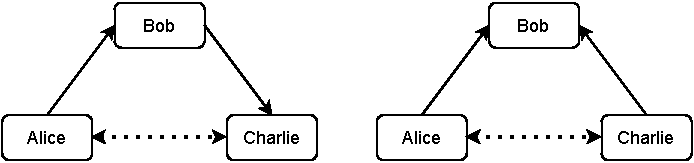
\includegraphics[width=\linewidth]{figures/transitiveBehavior.pdf}
  \caption{SSB transitive behaviors}
  \label{fig:transitiveBehavior}
\end{figure}


\section{Software}

SSB applications come in two parts: a server and a client. The server implements the actual protocol and has the task to replicate the messages between users and update the local database. The client accesses the database content, in general it implements a GUI for the users to see their content in a nice way. There exist multiple implementations of both. On the RPi, to demonstrate the device usage, we use sbb-server\footnote{Available at: \url{https://github.com/ssbc/ssb-server}}, the JavaScript reference implementation for a SSB server. We only use the server because a graphical interface is not necessary on the RPi. To properly verify the full functionality we also use the Oasis client\footnote{Available at: \url{https://github.com/fraction/oasis}} on other devices.

\section{Scenario: Follow Graphs}
\label{chap:followGraph}

To confirm the proper replication of users data and present the various possibilities that the device offers when used with the SSB protocol, we try out three scenarios with different initial follow graphs. To simplify the presentation of these follow graphs, we refer to a user by name, e.g. Alice, when we actually mean that user's main device, which has its own SSB identity. A follow from Alice to RPi\_A therefore means that Alice's main device's SSB identity follows the SSB identity
of RPi\_A. This section presents the three scenarios. In each of these scenario, informations should flow from one end user to the other.

The first example in \autoref{fig:singleRPi} only uses one RPi. It represents a situation where only one person in a group has the device and this person shares the Wi-Fi password with trusted people. Of course these connections can also be achieved through WPS with devices that implement it. It can also represent the situation where a single person wants to synchronize some data between several devices.

\begin{figure}
  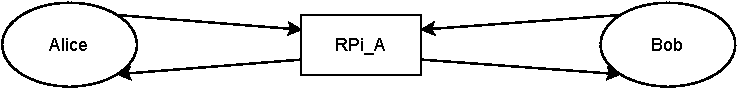
\includegraphics[width=\linewidth]{figures/singleRPi.pdf}
  \caption{Simple follow graph using a single RPi}
  \label{fig:singleRPi}
\end{figure}

The second example in \autoref{fig:transitive} shows a follow graph where Alice follows Bob, but their RPis do not know about each other. Exploiting the follow of a follow property of the SSB protocol, Alice's device receives data from Bob. But Bob can never receive any data from Alice.

\begin{figure}
  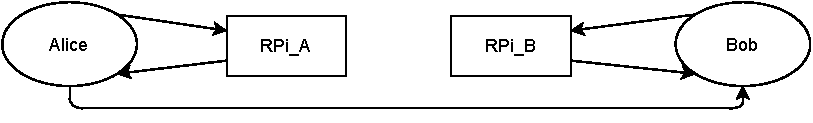
\includegraphics[width=\linewidth]{figures/transitive.pdf}
  \caption{Follow graph taking advantage of the transitive properties of SSB}
  \label{fig:transitive}
\end{figure}

The third and last example in \autoref{fig:multiplePeers} is a more complex follow graph where Bob uses multiple other devices with his RPi. But because Alice and Bob RPis follow each other, Alice can follow Bob's RPi and then discover all of Bob's devices.

\begin{figure}
  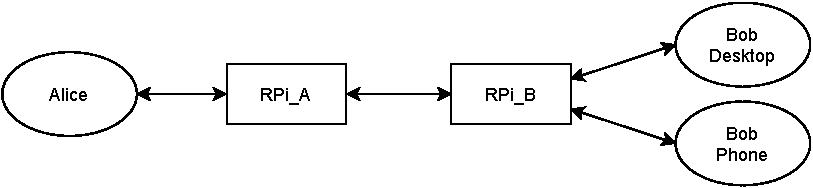
\includegraphics[width=\linewidth]{figures/complexGraph.pdf}
  \caption{Follow graph with multiple devices abstracted by a single RPi}
  \label{fig:multiplePeers}
\end{figure}



\section{Configuration}

Oasis and ssb-server use \emph{Node.js}\footnote{\label{foot:node}\url{https://nodejs.org/}} (Node). On the RPi, Node is already installed so only ssb-server has to be installed. The commands in \autoref{cmd:ssb_install} install ssb-server. Other devices can download Node on the Node website\textsuperscript{\ref{foot:node}}, then install and run Oasis with the commands in \autoref{cmd:oasis_install}.

\begin{figure}
\begin{lstlisting}[label=cmd:ssb_install, caption=Install and run ssb-server on the RPi]
    # This will install ssb-server in a ssb-server sub folder in the current folder:
    git clone https://github.com/ssbc/ssb-server.git
    cd ssb-server
    npm install
\end{lstlisting}
\end{figure}

\begin{figure}
\begin{lstlisting}[label=cmd:oasis_install, caption=Install and run Oasis on a device with Node.js]
    # Install Oasis (globally)
    npm -g install fraction/oasis
    # Run Oasis
    oasis
\end{lstlisting}
\end{figure}

Initially, the RPi and the other device do not follow each other. To have them follow each other, start both Oasis and the ssb-server. The ssb-server is started with line 2 of \autoref{cmd:ssb_run}. The command on line 3 of \autoref{cmd:ssb_run} lets the RPi follow the other device. The \verb|device_ID| is found under \emph{profile} on Oasis interface. From Oasis, under \emph{settings}, clicking on \emph{start networking} displays the RPi ID after some time. Clicking on it lets the user follow the RPi.

\begin{figure}
\begin{lstlisting}[ label=cmd:ssb_run, caption=Run ssb-server and follow, numbers=left]
    # From the ssb-server installation folder:
    node bin.js start&
    node bin.js publish --type contact --contact <device_ID> --following
\end{lstlisting}
\end{figure}

Additionally, to get situations like \autoref{fig:multiplePeers}, we use a script written for the project called \emph{ssbAutoFollow}\footnote{Also accessible on the smallworld repository: \url{https://github.com/rkuenzi-epfl/smallworld}}. This script makes the RPi follow any other device active on the same local network, using the fact that all ssb-server announce their identity on the local network by broadcasting UDP packets at regular intervals.

Finally, \autoref{conf:ssb_service} and \autoref{conf:follow_service} can be copied to \verb|/lib/systemd/system/| to have the ssb-server and the ssbAutoFollow script start on boot. The \verb|systemctl enable <service>| command also needs to be run for both services.


\begin{figure}
\begin{lstlisting}[language=bash, label=conf:ssb_service, caption=Service file for ssb-server, numbers=left]
    [Unit]
    Description=SSB server
    After=multi-user.target

    [Service]
    Type=simple
    User=pi
    StandardOutput=journal
    ExecStart=node <path-to-ssb-server>/bin.js start
    Restart=always

    [Install]
    WantedBy=multi-user.target
\end{lstlisting}
\end{figure}

\begin{figure}
\begin{lstlisting}[language=bash, label=conf:follow_service, caption=Service file for ssbAutoFollow, numbers=left]
    [Unit]
    Description=SSB auto follow
    After=multi-user.target

    [Service]
    Type=simple
    User=pi
    StandardOutput=journal
    WorkingDirectory=<path-to-ssb-server>/
    ExecStart=<path-to-ssb-server>/ssbAutoFollow
    Restart=always

    [Install]
    WantedBy=multi-user.target
\end{lstlisting}
\end{figure}


\section{Results}

This section illustrates how data effectively replicate between user devices in each of the scenario presented in \autoref{chap:followGraph}. For each scenario, we present one representative out of all possible sequence of connections that could lead to the same final state of data replication. In these diagrams, black dashed arrows indicate when a device connects to another, black arrows indicate when data get replicated from one device to another and red dashed arrows indicate when a device is disconnected from another.

\autoref{fig:replSinglRPi} demonstrates how the RPi gets the data from each user when they connect, using the follow graph of \autoref{fig:singleRPi}. If the RPi has some data that one of the user does not possess yet it sends these data to the user. In this scenario Alice and Bob do not follow each other, but they still exchange their data using the follow of a follow property. Now they have some data from one another so they can follow each other. Note that the same result is achieved if they both connect to the RPi at the same time. The only difference may be the order of replications.

\begin{figure}
  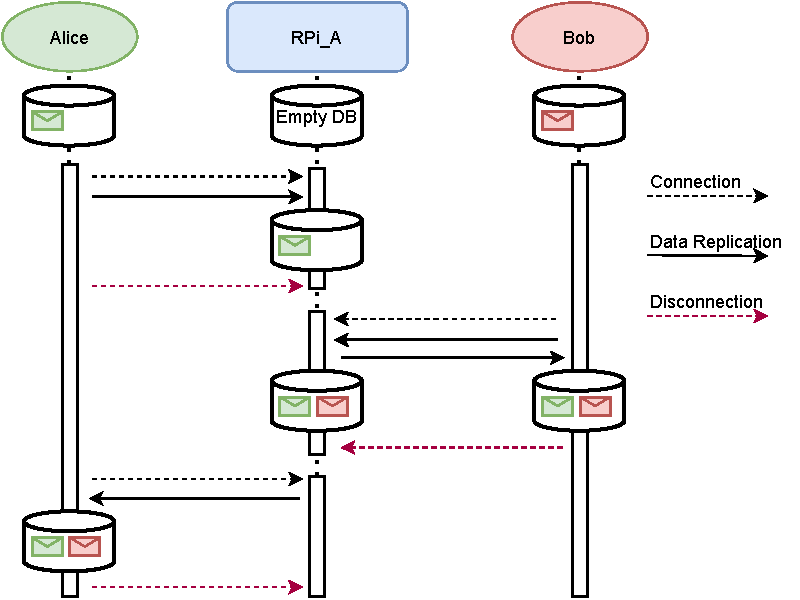
\includegraphics[height=10cm]{figures/replSingleRPi.pdf}
  \centering
  \caption{Data replication with a single RPi using the follow graph of \autoref{fig:singleRPi}}
  \label{fig:replSinglRPi}
\end{figure}


\autoref{fig:replTransitive} demonstrates how the transitive properties of SSB can help RPis replicate data of users who know each other, without the need for RPis to follow each other, which corresponds to the follow graph of \autoref{fig:transitive}. In this scenario, Alice's RPi does not follow Bob's RPi, but it knows that Alice follow Bob. According to the follow of a follow property, it means that Alice's RPi as an interest in Bob's data. Because of the common interest they have for Bob's data, when Alice's RPi connects to Bob's RPi, Bob's data get replicated to Alice's RPi. Alice can then retrieve Bob's data when she connects to her RPi. On the other hand, Bob's RPi does not replicate Alice's data because it does not have any interest in it.

\begin{figure}
  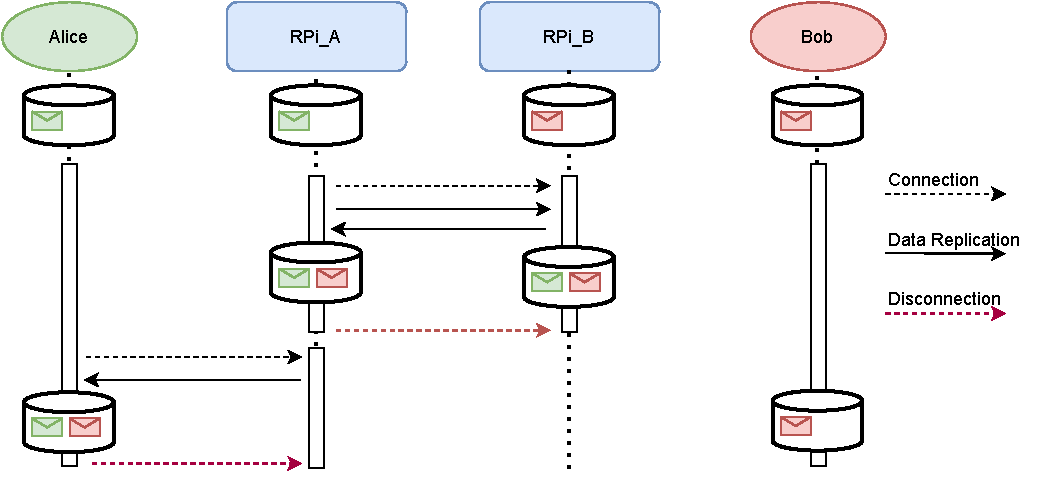
\includegraphics[width=\linewidth]{figures/replTransitive.pdf}
  \caption{Transitive data replication using the follow graph of \autoref{fig:transitive}}
  \label{fig:replTransitive}
\end{figure}

\autoref{fig:replComplex} demonstrates how the automatic follow script can help discover many other peers. At first in this scenario, Alice does not know anything about Bob, as presented by the follow graph of \autoref{fig:multiplePeers}. Because the RPis automatically follow one another when they connect, Alice's RPi gets all the data from Bob's devices by exploiting follow of a follow. Then Alice can decide to follow Bob's RPi. Once again taking advantage of the same property, Alice gets all the data from Bob's devices. From there she can decide to follow one or all of Bob's devices. The resulting follow graph is presented in \autoref{fig:complexFinal}.

\begin{figure}
  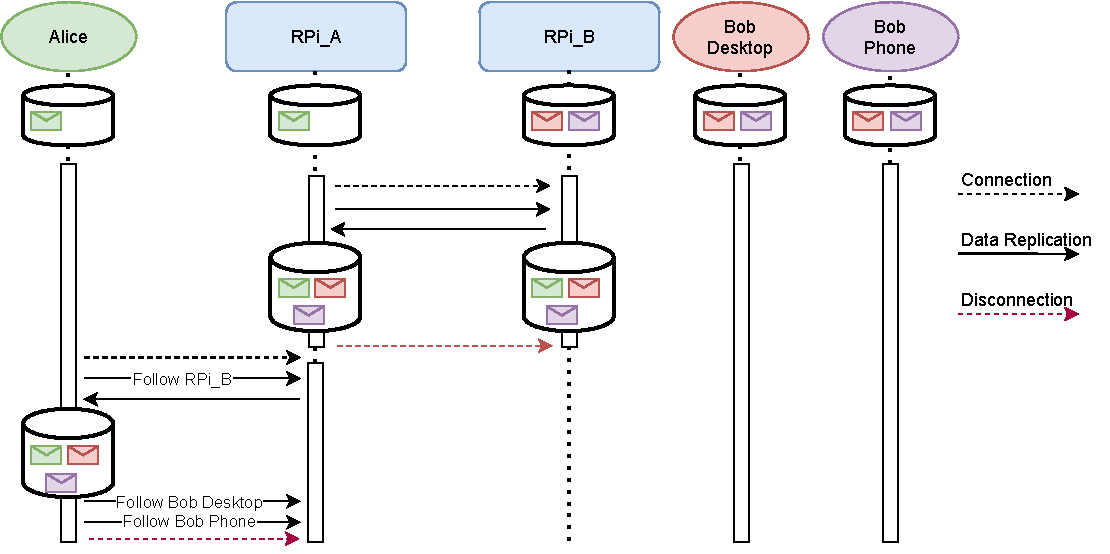
\includegraphics[width=\linewidth]{figures/replComplex.pdf}
  \caption{Data replication with RPi automatic follow using the follow graph of \autoref{fig:multiplePeers}}
  \label{fig:replComplex}
\end{figure}

\begin{figure}
  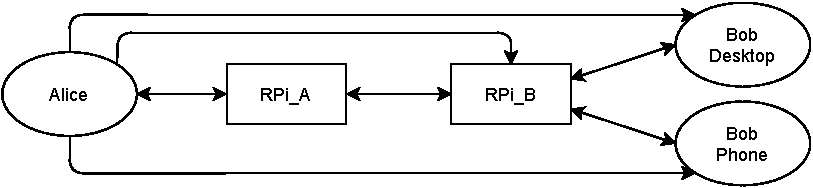
\includegraphics[width=\linewidth]{figures/complexFinal.pdf}
  \caption{Resulting follow graph taking advantage of automatic follow on RPis}
  \label{fig:complexFinal}
\end{figure}

\chapter{Another application: Dat Protocol}

Dat Protocol is a peer-to-peer protocol that allows sharing files in a distributed network.

It differs from BitTorrent in that contents can be updated by their author.


\section{Installation}

The installation of Dat is quite straightforward. The commands in \ref{cmd:dat_install} are used to install dat-cli.

It must be installed on both the emitter and the receiver devices.

\begin{figure}
  \begin{lstlisting}[label=cmd:dat_install, caption=Installing dat-cli]
    wget -qO- https://raw.githubusercontent.com/datproject/dat/master/download.sh | bash
    
    # or
    npm -g dat-cli
  \end{lstlisting}
\end{figure}

\section{Using dat}

The dat-cli command utility allows to simply interact with Dat files.

It is possible to create a shared folder using \emph{dat share} in the folder to share. This command will give a dat url starting with \emph{dat://} that can be used to retrieve the files on other clients.

A set of useful commands:
\begin{itemize}
  \item \emph{dat share}, to share a folder (starts a daemon that waits for incoming connexions)
  \item \emph{dat sync}, tries to retrieve newer version of the files, and share the files for incoming connexions
  \item \emph{dat clone <url> <folder>}, retrieves files from a dat url
  \item \emph{dat pull}, tries to retrieve a newer version of the files
\end{itemize}

\subsection{Real time synchronization with dat-share}

Dat does not directly provide a daemon to run in background and automatically synchronize folders for you. \\

A tool to do just that is \emph{dat-store}. It provides a service that can be run in background, can be remotely controlled, and does all the work for you.

It should be installed on both the client and the Raspberry Pi using 
\begin{lstlisting}
  npm -g dat-store
\end{lstlisting}

You should then configure a systemd service to run the store in background. The configuration on the user's device is 
\begin{figure}
  \begin{lstlisting}[label=cmd:dat_store_systemd_user, caption=Configure dat-store systemd service on the user device]
    
# This will create the service file.
sudo cat << EOF | sudo tee /etc/systemd/system/dat-store.service > /dev/null
[Unit]
Description=Dat storage provider, keeps dats alive in the background.

[Service]
Type=simple
# Check that dat-store is present at this location
# If it's not, replace the path with its location
ExecStart=$(which dat-store) run-service
Restart=always

[Install]
WantedBy=multi-user.target
EOF

sudo chmod 644 /etc/systemd/system/dat-store.service

sudo systemctl daemon-reload
sudo systemctl enable dat-store
sudo systemctl start dat-store

sudo systemctl status dat-store
  \end{lstlisting}
\end{figure}

\begin{lstlisting}
  npm -g dat-store
\end{lstlisting}

You should then configure a systemd service to run the store in background. The configuration on the user's device is done according to figure \ref{cmd:dat_store_systemd_user}. The configuration on the Raspberry Pi is achieved following figure \ref{cmd:dat_store_systemd_rasp}.

\begin{figure}
  \begin{lstlisting}[label=cmd:dat_store_systemd_rasp, caption=Configure dat-store systemd service on the raspberry pi]
    
# This will create the service file.
sudo cat << EOF | sudo tee /etc/systemd/system/dat-store.service > /dev/null
[Unit]
Description=Dat storage provider exposed to the internet (for the raspberry pi).

[Service]
Type=simple
# Check that dat-store is present at this location
# If it's not, replace the path with its location
ExecStart=$(which dat-store) run-service --expose-to-internet
Restart=always

[Install]
WantedBy=multi-user.target
EOF

sudo chmod 644 /etc/systemd/system/dat-store.service

sudo systemctl daemon-reload
sudo systemctl enable dat-store
sudo systemctl start dat-store

sudo systemctl status dat-store
  \end{lstlisting}
\end{figure}

Dat-store uses the concept of provider. Providers are instances of dat-store running either locally or remotely. The default one is your local instance, but you can also configure other providers, like the Raspberry Pi. \\
This notion is particularly useful for remote control of other providers. \\

Dat-store provides interesting commands that we will use in our demo:
\begin{itemize}
  \item \emph{dat-store add <url|path> [provider]}: Adds a folder or a dat url to the dat-store of the specified provider.
  \item \emph{dat-store set-provider <url> [provider]}: Sets the url of the specified provider.
  \item \emph{dat-store list [provider]}: Retrieves the list of available Dats in the specified provider.
  \item \emph{dat-store clone <path> <url> [provider]}: Clones \emph{<url>} into a local folder.
\end{itemize}

We can then imagine the case where we have two clients A and B and one Raspberry Pi used as a permanent store to synchronize a folder from A to B.

First, A executes the following commands:
\begin{lstlisting}[label=cmd:dat_store_example_A, caption=Commands executed by client A]

  dat-store set-provider http://raspberry.local:3472 raspberry
  mkdir mydat
  dat-store add ./mydat
  dat-store add ./mydat raspberry
\end{lstlisting}

Then, client B executes:
\begin{lstlisting}[label=cmd:dat_store_example_A, caption=Commands executed by client A]

  dat-store list raspberry
  dat-store clone ./mydat <url obtained from the previous command>
\end{lstlisting}


%%%%%%%%%%%%%%%%%%%%
\chapter{Conclusion}
%%%%%%%%%%%%%%%%%%%%

In this project, we designed and implemented Smallworld, an affordable device to simplify local peer-to-peer connectivity. The first step was to select which technology we would use. We settled on using Raspberry Pis for their low cost, and the multiple connectivity options they offered. This decision also allowed to focus on developping a single solution that is compatible with all existing devices, instead of trying to solve the incompatibility between them. Then we illustrated how users can use the device.

We implemented a solution for simple local peer-to-peer connectivity that works over Wi-Fi and Ethernet-over-USB in multiple steps. First, we selected relevant software tools, tested a number of possible configurations and explained those we retained. Second, we designed and implemented a user interface composed of two buttons and two LEDs in hardware, and a state machine that controls the behavior of the device in software which puts the device either in Wi-Fi host or client mode. The use of WPS greatly simplified the exchange of keys required to secure the connection. Third, we tested a wired connection to the device with Ethernet-over-USB, which for now only works with Linux laptops. Together, these steps enable any peer-to-peer applications that works with the Internet Protocol to communicate and replicate data with a Smallworld device.

The last step was to test that Smallworld could support a variety of replication scenarios of Secure Scuttlebutt (SSB), an existing peer-to-peer messaging application which transitively replicates data according to user-defined interests, as represented by follow graphs. We illustrated the data replication behavior for different follow graphs under representative connection scenarios. To simplify the initial configuration of those follow graphs, we have created a utility that automatically follows devices on the same local network, as happens when user or Smallworld devices are connected to one another.

\section{Possible Improvements and Future Work}

Our work builds a strong foundation upon which many improvements and extensions can be made. We list some of them in this section.

On the current device, the status of replication between devices is implicit. The device could provide an additional status LED, that would stay on while replication is in progress and turn off once replication is completed.

Because user may want more control over their device, a graphical user interface could also complement it. We can easily imagine two features that could be provided by such interface. The first one would let users have a better control over their follow graph, allowing them to choose who is followed and, as SSB also implements this feature, who is blocked by their Raspberry Pis. The second feature could give a more complete set of options to use the Wi-Fi controller. It could make it easier for users to add new Wi-Fi networks, and change their own network name and password. It could also allow to preserve the keys of trusted devices after a successful WPS connection.


\cleardoublepage
\phantomsection
\addcontentsline{toc}{chapter}{Bibliography}
\printbibliography

\end{document}
